% Created 2020-03-31 Tue 01:01
% Intended LaTeX compiler: pdflatex
\documentclass[11pt]{article}
\usepackage[utf8]{inputenc}
\usepackage[T1]{fontenc}
\usepackage{graphicx}
\usepackage{grffile}
\usepackage{longtable}
\usepackage{wrapfig}
\usepackage{rotating}
\usepackage[normalem]{ulem}
\usepackage{amsmath}
\usepackage{textcomp}
\usepackage{amssymb}
\usepackage{capt-of}
\usepackage{hyperref}
\author{Nuno Rodrigues A85207, Hugo Carvalho A85156, Hugo Ferreira A80665, João Faria A85632, João de Carvalho A83564, José Mendes A85951, José Miguel Alves Pires A50178\thanks{a50178@alunos.uminho.pt}}
\date{\today}
\title{Phase 1\\\medskip
\large Product concept, foreseen specifications, planning, tests and initial design}
\hypersetup{
 pdfauthor={Nuno Rodrigues A85207, Hugo Carvalho A85156, Hugo Ferreira A80665, João Faria A85632, João de Carvalho A83564, José Mendes A85951, José Miguel Alves Pires A50178},
 pdftitle={Phase 1},
 pdfkeywords={},
 pdfsubject={},
 pdfcreator={Emacs 26.3 (Org mode 9.3)}, 
 pdflang={English}}
\begin{document}

\maketitle
\tableofcontents


\section{Product concept: Radio Frequency Camera Assisted Rover (RFCAR)}
\label{sec:orgf4f2e51}
The envisioned product consists of a remote controlled car used to assist
exploration and maintenance domains. For this purpose, the vehicle should contain a
remotely operated camera feeding back video to the user. Additionally, the
vehicle must contain odometric sensors to assist in driving and prevent
crashes when user is not in control, e.g., when connection is lost.
The vehicle can be used for exploration of unaccessible areas to human operators
like fluid pipelines and other hazardous sites.

\section{Foreseen product specifications}
\label{sec:org942ed5c}
The foreseen product specifications are listed as topics below (sketch).

\subsection{Autonomy}
\label{sec:org7364ba5}
Check Battery and power consumption
\subsection{Velocity}
\label{sec:orgb41b31b}
Maximum Velocity allowed for the car
\subsection{Safety}
\label{sec:org4323985}
\begin{itemize}
\item Car: If the user issues a command that would cause damage to the system, the
system should take corrective measures to prevent it. The same holds true if
the communication between user and system is lost.
\begin{itemize}
\item \textbf{System uses odometric navigation}
\end{itemize}
\item Human: preserve human safety
\end{itemize}
\subsection{Image acquisition}
\label{sec:org7c6e617}
\subsubsection{Frame rate}
\label{sec:orgc44cea4}
\subsubsection{Range}
\label{sec:org7ecd940}
Camera's range
\subsubsection{Resolution}
\label{sec:orgb7a7db5}
\subsubsection{Color scale (Black and white or color)}
\label{sec:org8317faa}
\subsubsection{Always present or enabled on user command}
\label{sec:org64617a1}
\subsection{Usability}
\label{sec:org2063922}
\begin{itemize}
\item User-friendly interface
\item User interface responsiveness
\end{itemize}
\subsection{Load}
\label{sec:org1b54b04}
Maximum load the car can safely carry.
\subsection{Overall System latency/responsivess}
\label{sec:org826af3d}
The overall system latency is the sum of all systems' latencies, which must be
under a maximum tolerated value for the user.
\subsection{Communication}
\label{sec:org2a30eff}
\subsubsection{Reliability}
\label{sec:org16f237c}
Packet must be delivered (reliable, e.g. TCP) or not (e.g. UDP)
\subsubsection{Range}
\label{sec:org4411fa9}
Maximum distance allowed between user and system for communication purposes
\subsubsection{Transmission rate / throughput}
\label{sec:org521acaa}
\subsubsection{Redundancy}
\label{sec:org0bf292e}
\subsection{Sensibility}
\label{sec:orgc4bd738}
Sensibility to Smartphone motion
\subsubsection{Msg Smartphone->Raspberry}
\label{sec:org9772f2c}
x10 y20 v10
t5 v5

\noindent\rule{\textwidth}{0.5pt}
\subsection{Closed loop error (Control team)}
\label{sec:org6959821}
Error associated
\subsubsection{PI}
\label{sec:org560e9eb}
\subsubsection{PID}
\label{sec:org0f78f13}
\subsubsection{PD}
\label{sec:org3a6cfe5}

\subsection{Summary}
\label{sec:org322183a}
Table \ref{tab:specs-init} lista the foreseen product specifications.

% Please add the following required packages to your document preamble:
\begin{table}[!hbt]
\centering
\caption{Specifications}
\label{tab:specs-init}
\resizebox{\textwidth}{!}{%
\begin{tabular}{lll}
\hline
 & Values & Explanation \\ \hline
Max Velocity & 0.2 m/s & Maximum velocity of the conveyor belt in steady state \\ \hline
Dimensions & 60x30x30 cm & Dimensions of the conveyor belt in cm {[}l w h{]} \\ \hline
Time Min & 3 s & \begin{tabular}[c]{@{}l@{}}Time taken to transport a load the full extent \\ of the conveyor belt at maximum velocity\end{tabular} \\ \hline
Max Load & 1 Kg & \begin{tabular}[c]{@{}l@{}}Load the belt can hold without causing any \\ harm to the product\end{tabular} \\ \hline
Max slope & 15$^\circ$ & \begin{tabular}[c]{@{}l@{}}Maximum slope in which the conveyor belt can \\ operate at nominal conditions\end{tabular} \\ \hline
Slope levels & {[}0,5,10,15{]}$^\circ$ & Different levels of slope manually handled \\ \hline
Settling time & 0.2 $\cdot$ T & \begin{tabular}[c]{@{}l@{}}This means that it takes up to 20\% of the full \\ travel time to reach steady velocity\end{tabular} \\ \hline
Overshoot & 110\% Vss & \begin{tabular}[c]{@{}l@{}}Maximum velocity the conveyor belt reaches \\ before settling time\end{tabular} \\ \hline
Margin of error & 95\%-105\% of Vss & Admissible error in steady velocity \\ \hline
Power supply & 12V batteries, 6W & The main power supply will be 12V batteries \\ \hline
\end{tabular}%
}
\end{table}

\section{Planning}
\label{sec:org290d8c0}
In fig. \ref{fig:gantt-diag2} is illustrated the Gantt diagram for the project and in
fig. \ref{fig:gantt-tasks} the tasks' descriptions. It should be noted that the project
tasks of Analysis, Design, Implementation and Tests are performed in two
distinct iterations as corresponding to the Waterfall project methodology. The
tasks are described as follows:
\begin{itemize}
\item \uline{Project Kick-off}: in the project lift-off, the group is formed and the tutor
is chosen. A brainstorming about conceivable devices takes place, whose
viability is then assessed, resulting in the product concept definition
(Milestone 0).
\item \uline{State of the Art}: in this stage, the working principle of the device is
studied based on similar products and the system components and its
characteristics are identified.
\item \uline{Analysis}: In the first stage --- Analysis 1 --- contains the analysis
results of the state of the art. It should yield the specifications document,
containing the requisites and restrictions to the project/product, on a
quantifiable basis as required to initiate the design; for example, the
car maximum velocity must be, at maximum, \texttt{2 m/s}. The second stage --- Analysis 2
--- contains the analysis of the first iteration of the development cycle.
\item \uline{Design}: it is done in two segments: modules design --- where the modules are
designed; integration design --- where the interconnections between modules is
designed. It can be subdivided into \emph{conceptual design} and \emph{solution
design}. 
\begin{itemize}
\item In the conceptual design, several problem solutions are identified,
quantifying its relevance for the project through a measuring scale,
inserted into an evaluation matrix, for example, Quality Function Deployment
(QFD).
\item In the solution design, the selected solution is developed. It must include
the solution modelling, e.g.:
\begin{itemize}
\item Control system design: analytically and using simulation
\item Transducer design: circuit design and simulation
\item Power system design: power supply, motors actuation and respective
circuitry design and simulation
\item Software design: for all required modules, and considering its
interconnections.
\end{itemize}
\end{itemize}
\item \uline{Implementation}: product implementation which is done by \uline{modules} and
\uline{integrated}. In the first stage, the implementation is done in a prototyping
environment using breadboards, yielding prototype alpha; in the second stage
it must include the veroboards or Printed Circuit Boards (PCBs), yielding
prototype beta.
\item \uline{Tests}: unit tests --- \uline{by modules} --- and integrated tests are
performed. Tests are considered as those performed over any physical
component or prototype. It contains all the tests conducted into the system
and the several prototypes.
\item \uline{Verification/Validation}: after the alpha prototype is built the
specifications listed in the analysis must be verified and the prototype
validated by an external agent (an external user to the group).
\item \uline{Delivery}: --- project closure encompassing:
\begin{enumerate}
\item Final prototype built, verified and validated.
\item Support documentation: how to replicate, instruction manual.
\item Final report: \textit{<2020-06-18 Thu>}
\item Public presentation: \textit{<2020-06-19 Fri> }
\end{enumerate}
\end{itemize}

\begin{figure}[htbp]
\centering
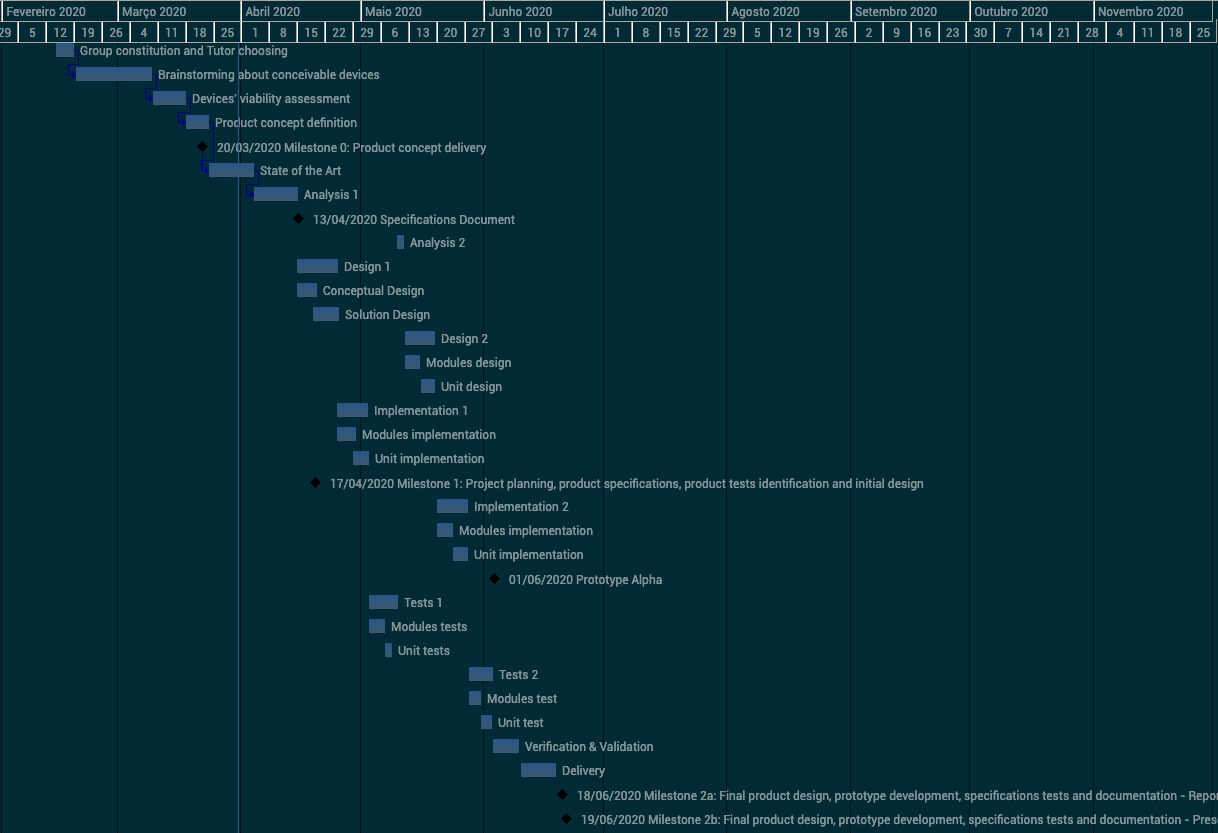
\includegraphics[width=1.0\textwidth]{../sec/img/gantt-diag-orig.png}
\caption{\label{fig:gantt-diag2}Project planning: Gantt diagram 1}
\end{figure}
\begin{figure}[htbp]
\centering
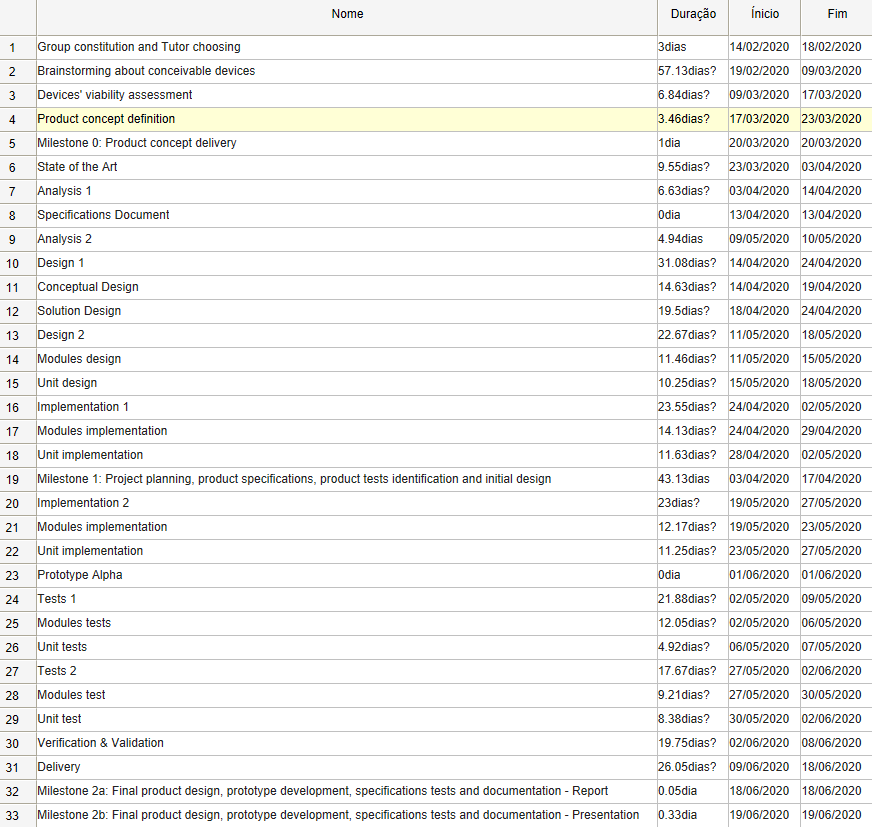
\includegraphics[width=1.0\textwidth]{../sec/img/gantt-orig-tasks.png}
\caption{\label{fig:gantt-tasks}Project planning: tasks}
\end{figure}

\section{Tests}
\label{sec:orga3bd3ad}
\subsection{Verifications tests}
\label{sec:orgab3743d}
The verifications tests are tests performed internally by the design team to
check the compliance of the foreseen specifications. These tests are done after
the prototype alpha is concluded.

\subsubsection{Maximum velocity}
\label{sec:org2d9e8e9}
The maximum velocity must be tested to ensure integrity of the
system. Furthermore, the degree of linearity of the velocity is respect to user
input must also be tested.

The procedure to test the maximum velocity is analogous to the velocity's
linearity trial, the only difference being the reference velocity’s regulation potentiometer position which should, for the maximum velocity’s case be at maximum.

The velocity of the conveyor belt can be measured internally to the system ---
measuring the induced voltage at the generator and converting to its physical
representation --- or externally using an tachometer for instantaneous value or
measuring the travel time and dividing by the conveyor length to obtain the
average velocity.

\uline{Internally}: The motor drives the conveyor belt at one end, also driving the
generator at the other end, due to their coupling. Thus, disregarding slip and
friction losses, the angular velocity of the motor and the generator are
identical. As \(\omega_m\) = \(\omega_g\) and \(v = \omega \cdot r\), the linear velocity of the conveyor can determined based on the angular velocity of the generator, which induces a proportional voltage at the terminals of the generator. Thus, by measuring this voltage, the linear velocity of the conveyor can be determined.

Using an oscilloscope to display the measured voltage at the generator and the
reference voltage, one will have the electrical representation of both the
desired velocity (physical representation of the reference voltage) and the
current velocity (physical representation of the voltage at the generator). 
One should see them as very similar, within a previously agreed upon range of
difference, accordingly to the type of controller used. This can be be used for
transient analysis of the conveyor's behaviour.

\uline{Externally} (instantaneous value): This first method will make use of the
physical relation between the linear velocity, v, the angular velocity,
\(\omega\), and the radius of the axis, r: \(v = \omega \cdot r\); and the previously
stated assumption that the conveyor’s linear velocity and the generator’s
angular velocity are directly proportional.

Using a tachometer to measure the motor's angular
velocity \(\omega\), the linear velocity of the conveyor belt can be determined,
through \(v= \omega \cdot r\), where \(r\) is the radius of the axis. 

Then through a comparison of the measured velocity and the physical representation of the reference voltage the outcome of the trial will be clear: if the velocities are similar within a range of difference that was agreed upon, it should be considered a success.

\uline{Externally} (average value): measuring the travel time (see Section
\ref{sec:orge574157}) of a part in the conveyor and
dividing by the conveyor length, the average velocity of the conveyor can be
determined. This can only be used for steady state analysis of the conveyor's
behaviour. Thus, if the average velocity is within the boundaries of the desired
velocity and the respective margin of error, the trial is considered a success.

For maximum assurance one should at least measure the velocity through the
internal method and one of the external followed by a comparison. This
comparison takes into account that for this procedure we agreed upon a 5\% margin
of error when comparing the measured and the reference velocities. It also
should consider the overshoot that will occur when the load is first placed,
which was agreed to be 10\%, therefore at any given time the conveyor’s velocity
should never surpass \texttt{0.2 m/s} (the agreed upon maximum velocity) \(\pm\) 10\%.

\subsubsection{Travel Time}
\label{sec:orge574157}
The time it takes a certain load with a constant mass to travel the full length
of the conveyor can be measured by a simple series of measurements using a
chronometer and the calculation of the average.

It should be noted that during the external measurement of velocity, the travel time was measured, there is a direct correlation between the two as such at assurance’s behest one should make sure that the results obtained during the velocity trial are in accordance with the values obtained in this procedure.

\subsubsection{Settling time}
\label{sec:orgc80717a}
The time that it takes the system to react to the presence of a load with a
constant mass and achieve a steady state.

The small scale of the conveyor and, consequently, its settling time (0.6
seconds minimum for the maximum velocity) dictate that the easiest method to
measure the conveyor velocity is by measuring the induced voltage in the
conveyor, capturing this data using the oscilloscope, this taking into account,
once again, the relation between the induced voltage at the generator and the
conveyor’s current velocity, as such by observing the induced voltage’s behavior
one can draw a conclusion regarding the settling time.

With the induced voltage at the generator captured by an oscilloscope,
specifically using the “single mode” present in these measuring instruments one
can observe the change that will occur in the generator’s voltage, more
specifically the moment a load is placed upon the running conveyor a change will
occur, the time it takes from this moment until the voltage returns to previous
value will be the settling time.

\subsubsection{Overshoot}
\label{sec:orgc7d8dd7}
An overshoot occurs when the output in a control system exceeds its final,
steady state value generally caused by a sudden change in the system, in this
case specifically, the placement of a load upon the conveyor will cause an
overshoot in the latter’s velocity which must be controlled lest it cause
problems.

An overshoot will occur during the settling time, as such, using the same
considerations taken in its measurement, it can be measured by observing the
induced voltage at the generator (an overshoot in the conveyor’s velocity will
correspond to a peak in the generator’s voltage).

Using an oscilloscope to display the induced voltage at the generator and making
use of the “single mode” present in these measuring instruments one can observe
the change that will occur in the generator’s induced voltage, the peak voltage
that will be seen when the load is placed upon the running conveyor is the
electrical representation of the overshoot of velocity, then either by
converting it to its physical representation or comparing it to the reference
voltage one can arrive at a conclusion. It was agreed that the overshoot
velocity should be \(V_{ss} \pm 10\%\), where \(V_{ss}\) is the stedy state velocity.

\subsection{Validation tests}
\label{sec:org36c46e4}
The validation tests should be performed by the client using the product’s
manual, so it is expected that a user without prior experience with the product
should be able to use it correctly and safely. 
For this purpose, a laboratory guide will be produced to work similarly to the
product’s manual, so the user can use the product also as a didactic kit. However, in this stage of the project, the laboratory guide hasn’t been prepared yet, but it’s already possible to have an idea about the type of tests and steps that will be necessary, such as:
\begin{itemize}
\item Motor tests;
\item Generator tests;
\item System parameter determination by measurements;
\item Tests using another controller;
\item Tests varying the load;
\item Tests changing slope levels;
\end{itemize}

\section{Initial design}
\label{sec:orgbc75a64}
After an analysis of the product's family tree (conveyors) and the
state of the art, an initial design of the product itself can be produced (see
fig. \ref{fig:initial-design}). 
The selected approach was top-down, in the sense that the
requisites and specifications were discussed and that resulted in a general
block diagram of the product concept. Some macro-level decisions were made
in this stage to narrow the problem's solutions pool, as follows:
\begin{itemize}
\item the product is a didactic kit about automatic control, therefore, the user
should be able to change the product's controller by any other that fits the
model. Thus, the controller's terminals should be user-accessible.
\item The product should be portable, thus, the main power supply source should be a
battery, which meets the DC motor power supply needs.
\item Power supply (\emph{PS}) should not restrict the usage of the product. Thus, the
user should be able to couple any DC power supply of his liking that meets the
product minimum power supply requirements (represented in the orange decision
block), in spite of the default battery existing in the prototype.
\end{itemize}

Additionally, a DC generator was included in the prototype design so
that the electrical representation of the DC motor velocity (or in other words,
a voltage) was measurable and later on converted to an actual velocity value by
analyzing the generator´s characteristic table. In other words, a table that
relates some measured voltage in the generator with its matching velocity value
in rpm (rotations per minute).

The measured voltage referred above and the command voltage represented
on the diagram in purple were also thought to be user-accessible via two
user terminals. This would allow some oscilloscope analysis afterwards.  
\begin{figure}[htbp]
\centering
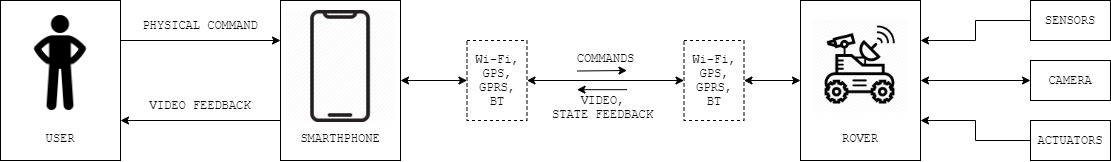
\includegraphics[width=1.0\textwidth]{../sec/img/initial-design.png}
\caption{\label{fig:initial-design}Initial design: Block diagram view}
\end{figure}

Thus, summarising, the initial design yields the system illustrated in
fig. \ref{fig:initial-design}, comprised of:
\begin{itemize}
\item \textbf{DC Motor}: the prototype provides a moving platform with a conveyor
belt driven by a direct current motor (\emph{Actuation Transducer});
\item \textbf{Controller}: generates the command variable (\emph{Manipulated Voltage})
according to its control rule, in this case, by taking the \emph{Measured
Voltage} as input;
\item \textbf{Generator}: the generator allows us to measure a voltage (electrical
representation of its speed [rpm] - \emph{Measured Voltage}) that will
later be converted to an estimated speed value;
\item \textbf{Amplifier}: with the \emph{Manipulated Voltage} as input the amplifier
generates an output voltage (\emph{Command Voltage}) that powers the
\emph{Actuation Transducer} (motor);
\item \textbf{Power Source}: powers the DC motor, the user has two options: using
any DC power supply that satisfies the motor power needs or using the
default battery power supply existing in the prototype;
\item \textbf{HMI}: a human-machine interface that allows the user to choose a
specific velocity magnitude and conveyor direction. Some LEDs will be
used later on to inform the user about the current charge of the
battery supply.
\end{itemize}
\end{document}